\subsection{Methodology}

\subsubsection{Waterfall}

{\bf The waterfall process: } is a sequential design process that 'flows' through the phases like a waterfall.
The waterfall process is also known as the 'standard' process because it was the most popular process before
agile processes became popular. 

With the waterfall process do only have a distinct goal for each phase. You can imagine a waterfall on the cliff of a steep moutian. Once the water is flowing over the edge of the cliff, it cannot turn back. It is the same with waterfall development. If you pick the first step of a normal waterfall process you will normally look at the analysis and requirement phase.

{\bf The phases in the waterfall:} there are five main phases in a normal waterfall process. We will here briefly
describe them:
\begin{itemize}
	\item {\bf Requirement specification:} is the phase where you collect all the requirement, functional and non-functional, to make a complete description of the behaviour of the system being developed.
	\item {\bf Design: } is the phase to take the requirements to make a overall design of the system like feks an
	architecture.
	\item {\bf Implementation: } is where the development of the designed system is done. In the implementation phase, 
	it is also normal to do some kind of testing.
	\item {\bf Verification (testing and installation): } when the implementation is done, the solution need to be tested and then installed.
	\item {\bf Maintainance: } is the modification of a software product after delivery to correct faults, to improve performance or other attributes.
\end{itemize}

\begin{figure}[ht!]
\centering
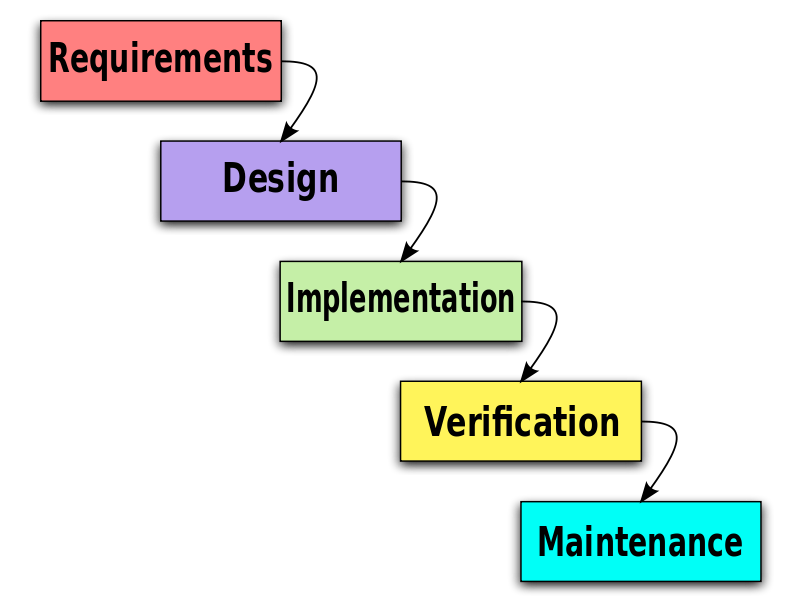
\includegraphics[scale=0.3]{pictures/Waterfall_model.png}
\caption{The waterfall process}
\label{overflow}
\end{figure}

{\bf Pros: }
\begin{itemize}
	\item Simple and easy to understand and use
	\item Phases are processed and completed one at a time.
	\item Works in projects where the requirements are well understood (low risk for changing the requirements)
\end{itemize}

{\bf Cons: }
\begin{itemize}
	\item It is very difficult to change the requirement specification, so it is not suitable for the projects where requirements are at a moderate to high risk of changing.
	\item No delivery of working software until the of the process. This can be critical because the customers may not
	be able to be a part of the process and can entail a unhappy customer.
	\item 
\end{itemize}

{\bf When to use a waterfall process?: }




\subsubsection{Scrum}
{\bf The Scrum process: } Scrum is a agile iterative process with focus on small deliveries. The process
defines a self-sustaining team ("The scrum team") that defines the goal for each phase. The goal 
is achived through small product increments in iteration that normally last for 1-4 weeks. 
All the functions to implement is planned and is added to a listcalled a "Product Backlog". The
functions is normally defined as userstories and is added in a prioritized order. In each inkrement, 
in scrum called a "Sprint", there is a sprint meeting where the scrum team pick userstories from the 
product backlog and add them to a "Sprint Backlog". The sprint backlog is the description of what 
to deliver in the end of the sprint.

Since it is a flat structure there is a concept in scrum called "daily standup". This will keep
the team together and everyone will be able to get a quick status update and is normally lasting
for only 5-15 minutes. 

In a scrum process the stakeholders are a part of the team. The stakeholders will be able to give
feedback in every sprint in terms of changes or approval of a delivery in what is called a "sprint review".
In other methodologies, the stakeholders are only a part of a big delivery in the end, and will 
make it difficult to make changes to what is developed. In scrum, each sprint is a small delivery.

{\bf Pros: }
\begin{itemize}
	\item Small deliveries with feedback from stakeholders
	\item Oppertunity to make changes to the requirements during the process
	\item Flat structure (this will adapt to small and bigger teams)
	\item Daily status update from daily standup meetings
	\item Fits for small teams
\end{itemize}

{\bf Cons: }
\begin{itemize}
	\item Require the stakeholders (the customer) to be a part of the team and participate during the process.
\end{itemize}

\subsubsection{Conclusions}
In this section we have described to different methodologies that we considered as a possible solution 
for our project. Since our project is to develop a game with few requirements from the customer, we are
depending on a process that will adapt to constant changes in the requirement specification. 
In the waterfall process, it will not support this and it will be hard for us to be able to use a
such process. The scrum process is more likely to fit our project in terms of amout of planning, 
number of team members and also the high possibility for changes on the requirements.


% http://en.wikipedia.org/wiki/Waterfall_model
% http://searchsoftwarequality.techtarget.com/definition/waterfall-model
% http://en.wikipedia.org/wiki/Kanban_(development)
% http://www.djaa.com/principles-kanban-method
